%----------------------------------------------------------------------------------------
%	Section: The problem
%----------------------------------------------------------------------------------------
%\lettrine[nindent=0.3em,lines=3]{K}%
Kidneys, although often underestimated, are fundamental organs of human body and their working mechanism is extremely complex. Their essential task is to remove wastes from the organism but their functionality is much wider. They are also involved in maintaining acid-based balance, regulating the blood pressure and are major endocrine organs, which secret three important hormones: erythropoietin, calcitriol and renin. Besides the production, they also take part in degradation of hormones such as insulin or parathyroid hormon \cite{saladin}.
The basic functional units of the kidney are nephrones. Above million of them enables it to perform above functions \cite{health_and_disease}.
  
Anatomically, kidney can be divided into three main parts:
\begin{inparaenum}[(1\upshape)]
\item renal cortex, which is the outer part of the kidney
\item medulla, the inner part of the kidney composed of medullary pyramids
\item pelvis, the extension of the ureter, which collects the urine \cite{saladin, health_and_disease}. The structure of the kidney is shown on Figure \ref{fig:kidney_anatomy}.
\end{inparaenum}

\begin{figure*}
	\centering
	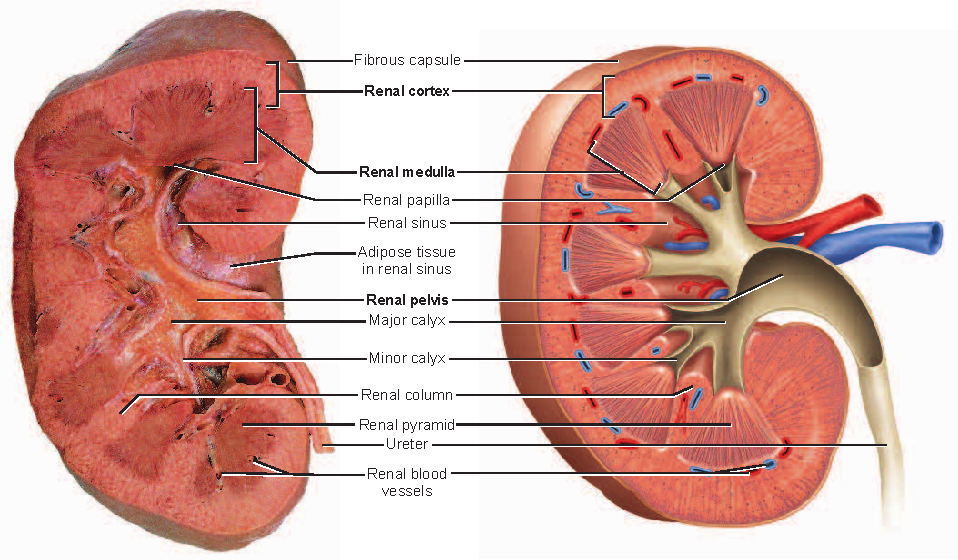
\includegraphics[height = 8cm]{img/kidney}
	\caption{Anatomy of the kidney \cite{saladin}.}
	\label{fig:kidney_anatomy}
\end{figure*}


Kidneys are responsible for maintaining homeostasis of all body due to which, all organs can work in optimal environment.
It is crucial for proper functioning of whole organism \cite{mosby}. One can conclude that the role of kidneys is enormously important. 

Gradually progressing loss of kidney function known as a chronic kidney desease is a~ growing world-wide problem. As much as 8--16\% of whole population suffers from this condition \cite{statistics}. It significantly decreases comfort of life and in extreme cases leads to death. What is more, it was shown that renal diseases are risk factor for development of cardiovascular diseases \cite{cardiovascular_diseases}.
Because of the fact that symptoms don't resemble renal failure, approximately 90\% of the ill are unconscious of it until late stages \cite{national_kidney_foundation}. That is way there is the demand for methods, which enable fast and accurate measurement of renal function required for all of three: prevention, monitoring and therapy.   

\subsection{Glomelural Filtration Rate}
The metrics of level of kidney function is glomelural filtration rate (GFR) \cite{traynor2006measure}. Not only does it allow for assessment how well our kidneys are working, but also it can determine the stage of kidney disease. In short terms, it is the volume of fluid filtered from the renal glomerular capillaries into the Bowman's capsule per unit time \cite{gfr_dictionary}. %It corresponds to to the Clearance Rate when any solute is freely filtered and is neither reabsorbed nor secreted by the kidneys.%
GFR measurement is of great clinical importance and is crucial for diagnosis and management of renal diseases.
The GFR in healthy adult kidney is equal approximately 90--130 mL/min/1.73 m\textsuperscript{2} \cite{normal_values}. Lower at birth, it approaches its adult value at the age two and maintains its level till the age of fourty, when it starts decreasing again \cite{weinstein2010aging}.     

The classical method of GFR measurement incorporates injection of the exogenous marker that is freely filtered by the kidney, and that does not undergo metabolism, tubular secretion or absorption. An example of such a~marker can be insulin, ohexol or iothalamate. 
Even thought this method is considered the gold standard in GFR measurement, because of its limitations, it is not a clinical routine if very accurate measurements are not required. This special cases include transplant donors or scientific research \cite{traynor2006measure}. 
Other, more frequently used techniques involve using endogenous markers such a creatinine or urea and estimating GFR applying validated algoritms \cite{delanaye2012measuring}.

Although described methods allow for sufficiently accurate GFR estimation or even exact measurement, they are not very practical in clinical use. 
Not only are they time-consuming and expensive but also they can be cumbersome. What is more they cannot be used for single kidney function assessment and thus other methods are desired \cite{bokacheva2008assessment}.

\subsection{DCE-MRI of the kidneys}
An innovative approach in estimating renal function is performing dynamic contrast-enhanced magnetic resonance (DCE-MRI). During the examination a contrast agent is injected into the blood and the T1-weighted images are acquired. The passage of the tracer through the kidney results in changes in signal intensities over the time.
The analysis of the obtained time-intensity changes as a function of time provides important functional information \cite{bokacheva2008assessment, khalifa2014models}. Traditionally, this evaluation is performed by experienced observer, although this method is very subjective and strongly depends on the experience of the expert. Other technique involves fitting tissue intensity changes to pharmacokinetic models, which allows quantification of renal function \cite{khalifa2014models}. Even though this strategy is gaining more and more supporters, most of the methods still require interference of the human at some stage, which makes them vulnerable to human factors. 


\subsection{Aim of the overall project}
The overarching aim of this project is to develop entirely data-driven method of GFR estimation directly from DCE-MRI, which would be fast and efficient and accurate enough to be used it clinical applications.  
